\chapter{建立計算工作流}\label{ch:workflows}
\index{Gongzuoliu@工作流}

工作流把結構準備、電子結構求解和結果顯示組織為一張可以閱讀和重複執行的圖。它既適合一次簡單的 SCF，也適合把對稱性分析、能帶、態密度和結構最佳化串成一套計算過程。本章先介紹編輯方法，再用矽晶體和氫分子完成幾條常用工作流。

如果已經完成第\ref{ch:first}章，可以從本章的矽教程繼續。配套專案 \file{examples/silicon-tutorial.ks} 提供八原子矽晶胞的 SCF 與 DOS，\file{examples/silicon-band-primitive.ks} 提供二原子矽原胞的能帶與對稱性工作流，\file{examples/h2-tutorial.ks} 提供氫分子的 SCF 與結構最佳化。專案中同時儲存了示例計算結果，可先檢視，再重新執行。

\section{編輯工作流}

\subsection{節點怎樣組織任務}
\index{Gongzuoliu jiedian@工作流節點}

畫布上的一個節點代表一項任務。選擇節點後，再選擇 \ui{工作流 → 配置節點}，或使用節點上的齒輪，展開右側的 \ui{配置編輯器}，開啟或重新整理該任務的專用 \ui{選項}。向下滾動即可檢視具體引數。本章下文的“配置某節點”均採用這一操作。模組按處理階段組織功能，任務決定節點實際做什麼。標籤只是畫布上的名稱，可以改成更容易識別的表述。

例如，一個標籤為“建立矽模型”的節點可以執行 \ui{Build Molecule}；標籤為“電子自洽”的節點執行 \ui{SCF}。修改標籤不會自動修改任務型別。初次建立工作流時，先選擇正確的任務，再決定是否需要重新命名。

連線表示處理順序。下游任務需要上游準備好的資料，能帶計算需要自洽密度和路徑，收斂圖需要迭代歷史。連線不應形成迴圈；幾何最佳化中的重複求解已經由最佳化任務內部完成，不需要在畫布上把最佳化節點連回自身。

\subsection{選擇起始工作流}

\ui{從模板建立工作流} 中提供 SCF、Energy Band、DOS、Relaxation 和 Symmetry。模板適合學習常見任務的組合方式。開啟後，選擇要計算的結構並檢查引數，再執行工作流。一個專案包含多個結構時，應在結構輸入節點中明確選擇計算物件。

從空白建立更適合定製流程。可以新增節點、調整輸入輸出埠、連線節點，再為每個節點指定任務。編輯畫布時，可以利用縮放、適配檢視、撤銷和重做整理佈局。清楚的佈局便於檢視節點之間的關係。

\begin{steps}
\item 新建空白工作流，新增第一個節點。
\item 選擇節點，使用 \ui{工作流 → 配置節點} 展開配置編輯器，再設定所屬模組和任務。
\item 繼續新增下一個節點，並按資料處理順序連線。
\item 逐一配置結構、物理引數和數值引數。
\item 給工作流命名並儲存，然後從小規模計算開始驗證。
\end{steps}

\subsection{儲存專案與儲存工作流的區別}

專案檔案 \file{.ks} 儲存結構、工作流和結果等整套內容。工作流檔案 \file{.wf} 儲存一張流程圖及其中的任務設定，適合在不同專案之間複用計算方法。與他人分享 \file{.wf} 檔案時，還需提供對應結構，並說明如何選擇結構輸入。

日常使用時，儲存專案可保留完整計算內容。需要在其他體系上覆用一套計算方法時，再將流程儲存為工作流模板，並根據新體系調整結構和精度設定。


\section{選擇任務}\label{sec:task-catalog}

模板覆蓋常用組合，任務列表則列出可放入節點的具體工作。節點所屬的\ui{模組}先確定處理階段，\ui{任務}下拉框再選擇功能。一個節點執行一種任務，任務型別在配置編輯器中選擇。

\begin{longtable}{p{.28\linewidth}p{.65\linewidth}}
\caption{工作流任務及其作用。}\label{tab:task-catalog}\\
\toprule
模組與任務 & 用途和需要先準備的內容 \\
\midrule
\endfirsthead
\toprule
模組與任務 & 用途和需要先準備的內容（續） \\
\midrule
\endhead
Preprocessing & \ui{Symmetry \& K-Path}：分析晶體對稱性併產生高對稱路徑；輸入選定的晶體結構。 \\
Computation & \ui{Build Molecule}：將專案結構轉為計算物件，設定泛函、贗勢、截斷與取樣。 \\
Computation & \ui{SCF}：尋找自洽電子密度，產生基態能量、電子態和迭代歷史。 \\
Computation & \ui{NSCF}：準備非自洽求解選項，供後續能帶或DOS任務採用；單獨執行該節點不會生成新的能帶圖。 \\
Computation & \ui{Geometry Optimization}：在電子計算基礎上改變原子位置；需要完整的基態計算條件。 \\
Computation & \ui{TDDFT}：由基態電子態準備Casida激發態計算；引數與求解方法見本章激發態小節。 \\
Postprocessing & \ui{Band Calculation}：沿高對稱路徑生成k點並進行非自洽計算；需要SCF結果、NSCF選項和對稱性路徑。 \\
Postprocessing & \ui{Band Calculation 3D}：在選定倒空間平面上取樣；需要SCF結果和NSCF選項。 \\
Visualization & \ui{Energy Curve}：把SCF能量與誤差歷史繪為收斂圖。 \\
Visualization & \ui{Band Structure}：繪製路徑能帶，讀取Band Calculation結果。 \\
Visualization & \ui{Band Structure 3D}：繪製取樣平面上的能量曲面，讀取Band Calculation 3D結果。 \\
Visualization & \ui{DOS}：採用NSCF網格計算並顯示總態密度。 \\
Visualization & \ui{Brillouin Zone 2D}：顯示二維布里淵區及路徑，讀取對稱性分析結果。 \\
Visualization & \ui{Brillouin Zone 3D}：顯示三維布里淵區及路徑，讀取對稱性分析結果。 \\
\bottomrule
\end{longtable}

表中的任務名與列表中的英文一致。前處理回答“模型和路徑怎樣定義”，計算任務準備電子結構，後處理在所得電子態上繼續取樣，視覺化把已有資料變成圖。DOS還在自身任務中進行網格取樣，因此不能只按模組名稱推斷它是否需要數值計算。

\section{為節點新增埠}

節點上方的埠接受前序連線，下方的埠連線後續節點。\ui{0-0 節點}沒有上下埠，\ui{0-1 節點}只有下埠，\ui{1-0 節點}只有上埠，\ui{1-1 節點}上下各有一個。它們描述的是畫布連線形式，不是四種不同求解器。

\begin{steps}
\item 啟用一張空白工作流，開啟\ui{工作流 → 新增節點}的下拉選單，先新增一個\ui{0-1 節點}。
\item 將它配置為\ui{Computation Module → Build Molecule}，選擇已經匯入的結構。
\item 再新增兩個\ui{1-1 節點}，分別配置為\ui{SCF}和\ui{Energy Curve}，後者屬於\ui{Visualization Module}。
\item 從前一個節點下方的埠拖動到後一個節點上方埠，依次連好三個節點。
\item 若選錯埠形式，選中節點後用\ui{編輯節點}中的新增或移除上、下埠調整；刪除仍在使用的埠前，先核對連線。
\item 用\ui{放大}、\ui{縮小}和\ui{適配檢視}看清整個流程，再儲存專案。
\end{steps}

完成連線後，檢查每個節點的任務與引數，然後執行SCF工作流。撤銷和重做可以恢復畫布編輯；儲存\file{.wf}便於下次在另一個專案匯入同一流程。

\section{讀懂節點的通用設定}

配置節點時，\ui{通用}用於標籤、模組和任務；\ui{選項}與\ui{高階選項}才是該任務的計算引數。更換任務會換成另一組引數，不會自動把前一種任務的設定逐項轉換過去。先選擇任務，再填寫對應引數。

\ui{輸入}、\ui{資源}和\ui{輸出}也在編輯器中顯示。\ui{資源}中的並行環境、程序數與執行緒數會參與實際執行；輸入訪問、輸出儲存與傳遞的勾選項，以及資源中的\ui{時間限制}，不執行結果篩選或自動中止。執行結果可在\ui{Results}中檢視，儲存專案即可保留。

\section{為計算節點分配資源}\label{sec:node-resources}
\index{Bingxing jisuan@平行計算}

\subsection{先區分節點順序與節點內部的並行}

工作流按連線確定的先後關係依次執行節點。把畫布畫成兩條分支，並不會讓兩條分支同時計算。節點內部的並行則把一項任務中的部分數值工作分給多個計算程序，例如在非自洽計算中分配不同的k點。兩者的設定與作用各不相同。

配置入口位於當前節點的\ui{資源}面板。先選節點，再點選\ui{工作流 → 配置節點}，展開\ui{資源}，便可檢視這個任務允許採用的執行方式。可選方式隨任務與\ui{DiagMethod}所選的對角化方法改變。

\begin{table}[!htb]
\centering
\caption{節點資源欄位的含義。}
\label{tab:node-resource-fields}
\begin{tabularx}{\linewidth}{lX}
\toprule
欄位 & 如何理解與填寫 \\
\midrule
並行環境 & 選擇\ui{序列}、\ui{並行（程序池）}、\ui{GPU（對角化）}，或在支援的後續任務中\ui{繼承 NSCF 配置}。實際可選項由當前任務決定。\\
最大程序數 & 正整數，預設2；限制程序池的Worker數。僅在程序池模式下可編輯。\\
執行緒/程序 & 正整數，預設1；限制每個計算程序的CPU計算執行緒數。可在程序池或GPU模式下編輯。\\
時間限制 & 可見No Limit、30 minutes、1 hour、2 hours；此欄位不觸發自動停止。\\
\bottomrule
\end{tabularx}
\end{table}

一個Worker是參與運算的計算程序。假設設定最大程序數2、執行緒/程序1，意思是最多使用兩個Worker，每個Worker最多使用一個CPU計算執行緒。主應用本身還需要執行介面和安排任務，因此這兩個數不能直接當作作業系統中全部程序與執行緒的總數。增加Worker也會增加記憶體佔用，小型練習未必更快。

\ui{序列}表示這一節點不啟用程序池或GPU計算，並不強制CPU只使用一個核心；數值庫仍可能使用自身的CPU執行緒。\ui{執行緒/程序}也不是執行緒型並行池的開關。節點程序池使用程序型Worker。

\subsection{檢視當前任務支援的方式}

\begin{table}[!htb]
\centering
\caption{常用任務的資源選擇。}
\label{tab:node-resource-support}
\begin{tabularx}{\linewidth}{p{.29\linewidth}X}
\toprule
任務 & 當前可以選擇的方式 \\
\midrule
SCF & 序列；採用受支援的對角化方法時可選GPU。此節點不提供程序池並行。\\
NSCF & 序列；關閉HT插值時可用程序池，並在方法受支援時可選GPU。這裡儲存的資源可由後續能帶與DOS任務繼承。\\
Band Calculation、DOS & 序列、繼承NSCF、程序池，以及受方法支援的GPU。啟用HT插值時不提供程序池或GPU。\\
Band Calculation 3D & 序列、繼承NSCF、程序池，以及受方法支援的GPU；此任務直接進行NSCF取樣，不採用HT插值。\\
其餘任務 & 當前資源列表為序列，包括結構建立、對稱性分析、幾何最佳化、TDDFT及一般繪圖任務。\\
\bottomrule
\end{tabularx}
\end{table}

GPU選項適用於\texttt{lobpcg}、\texttt{davidson}、\texttt{davidson2}和\texttt{davpcg}這些對角化方法。SCF預設的\texttt{davidson\_qe}不在此列，因此初次開啟SCF資源面板時可能只見序列。GPU加速用於受支援的對角化步驟，其他計算與繪圖仍按各自的執行方式執行。GPU模式中的\ui{執行緒/程序}限制CPU端計算執行緒，GPU核心執行緒由裝置管理。

能帶和DOS採用前序NSCF節點的對角化選項，因此判斷其資源選擇時，也要檢查NSCF的\ui{DiagMethod}與\ui{Use HT}。修改任務或方法後，原先不再適用的資源選擇可能恢復為序列；執行前重新開啟資源面板核對一次。後續節點採用\ui{繼承 NSCF 配置}時，顯示繼承的程序與執行緒數量，兩個數值框不可直接編輯。需要改變它們，應返回NSCF，或在後續節點選擇自己的執行方式。

一張工作流中若放置多個NSCF節點，後續取樣採用執行順序中最近一次經過的NSCF配置；它不按畫布上的距離選擇，也不分別為每條分支儲存一套獨立配置。需要比較不同資源或求解條件時，可先各儲存一張工作流，使每次繼承的來源清楚。

\subsection{練習：給矽\headinglatin{DOS}設定兩個\headinglatin{Worker}}

這項練習沿用本章的矽DOS工作流，不改變結構、截斷能、k點網格、能量範圍或步長。先完成序列參考執行，再比較另一種執行方式，較容易判斷差別來自計算條件還是執行環境。

\begin{steps}
\item 開啟矽DOS工作流，選擇\ui{NSCF}節點，點選\ui{配置節點}。
\item 在\ui{選項}中保持\ui{DiagMethod}為\texttt{lobpcg}，並使\ui{Use HT}保持關閉。
\item 展開\ui{資源}，把\ui{並行環境}改為\ui{並行（程序池）}；填寫\ui{最大程序數}為2、\ui{執行緒/程序}為1。
\item 選擇\ui{DOS}節點，檢視其資源面板，選擇\ui{繼承 NSCF 配置}，核對顯示的數量為2和1。
\item 儲存專案。在執行環境提供相應並行能力後執行整張工作流，檢視日誌中的k點計算資訊，再檢查新產生的DOS結果。
\item 記錄本次資源設定和用時。如需恢復序列比較，將NSCF改為\ui{序列}，再核對DOS仍然繼承該設定。
\end{steps}

NSCF節點主要準備求解選項，不在這一節點上完成整條能帶或DOS取樣。真正使用程序池的是後續進行非自洽求解的任務。k點數大於1時，受支援的k點迴圈才會分給多個Worker；只在單一k點上計算，不能據此期待獲得相同的並行收益。選擇\ui{序列}會關閉本次節點的程序池計算路徑，但保留已有並行池。

資源設定不改變所要求解的物理模型。比較結果時，仍須核對收斂、取樣及能量參照；不同執行方式可能產生數值末位的差別。第一次建立並行池所需的時間也應與實際求解時間分開理解。


\begin{figure}[!htb]
\centering
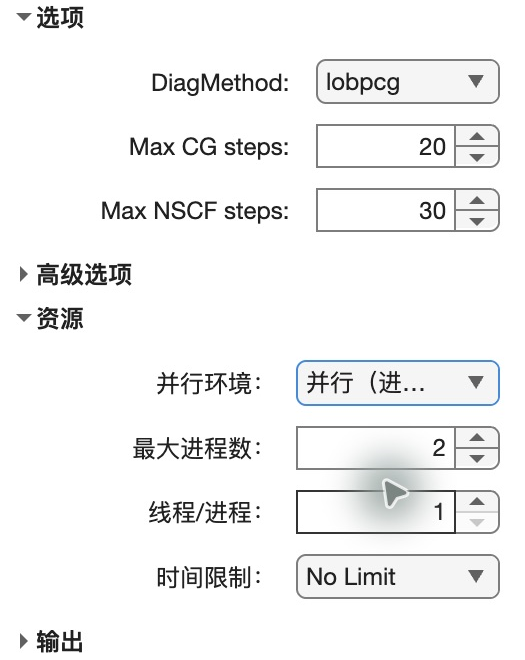
\includegraphics[width=66mm]{publication-assets/revision-nscf-process-resources.png}
\caption{NSCF節點的資源設定區域性：選擇程序池，最多兩個Worker，每個Worker一個CPU計算執行緒。}
\label{fig:nscf-resources-live}
\end{figure}

\begin{figure}[!htb]
\centering
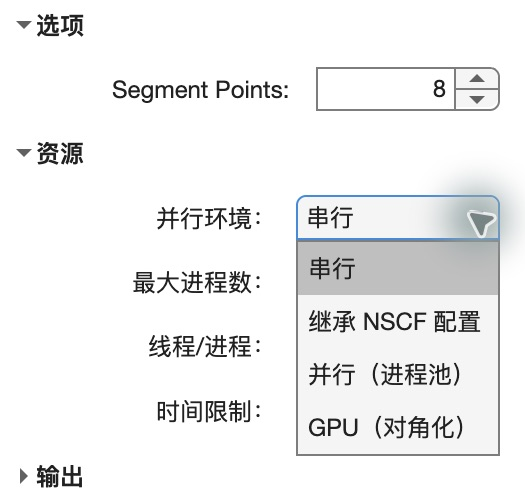
\includegraphics[width=70mm]{publication-assets/revision-band-resource-options.png}
\caption{Band Calculation節點提供繼承NSCF配置的選項，也可另選自己的執行方式。}
\label{fig:band-inherit-live}
\end{figure}

\FloatBarrier
\subsection{處理資源不可用的提示}

下拉框中的一種方式表示任務支援這種計算路徑，執行時還要檢查執行機器的環境。程序池需要可用的Parallel Computing Toolbox與程序型池配置；GPU需要可用且受支援的GPU及相應計算元件。瀏覽器中的畫面在個人電腦上顯示，計算資源卻由執行應用的伺服器提供。線上版首頁的\ui{並行}按鈕禁用，不等於節點資源面板中的並行一律不可用；能否執行，應看節點選擇及伺服器實際提供的環境。

如果還沒有池，應用會嘗試按節點的\ui{最大程序數}建立本地程序池。請求的程序數超過本地配置允許的Worker數時，會報告數量超限，不會自行改成更大的池。如果已有池，程式會檢查池的型別、Worker數與每個Worker的CPU執行緒數；執行緒型池、超過節點上限的池，或執行緒數超過限制的池，都會產生衝突提示。已有且滿足限制的較小池可以繼續使用，\ui{最大程序數}不保證每次都新建恰好這麼多Worker。

尚未配置並行環境時，可先把節點改為序列，完成小型練習，再核對執行環境。完整MATLAB\regmark{}使用者若自行建立過池，可先關閉不相容的池，再按節點設定執行；應用保留使用者已有池的配置。由當前節點自行建立的臨時池，會在該任務結束或退出時釋放。

\subsection{把節點設定帶到遠端環境}

節點資源決定任務怎樣使用計算資源；第\ref{ch:remote}章的遠端配置決定任務提交到哪裡。這兩項可以同時使用，但填寫兩個Worker不會自動把任務送到叢集，也不會改變節點的先後順序。

遠端提交會攜帶節點資源設定。遠端作業已經執行在Worker中時，不能再依靠節點臨時建立一個巢狀程序池；需在提交作業時預留滿足節點限制的程序池，並使遠端Worker的執行緒數相容。例如節點限制為最多2個Worker、每個1執行緒，遠端已有4個Worker的池就不符合這個上限。叢集配置中的Worker數量、PoolSize和節點中的限制應一起檢查。

線上版狀態列的CPU與記憶體讀數用於觀察當前會話，不是資源申請按鈕。儲存專案時一併儲存節點設定；記錄遠端計算時，還應保留所選叢集及提交條件，以便下次在同一環境復現。


\section{矽晶體：建立第一個週期計算}

\subsection{準備八原子矽晶胞}

矽是理解週期計算和半導體能帶的良好例子。本教程使用包含八個矽原子的立方晶胞，晶格常數為 $5.4437023729$ Å，結構儲存在 \file{examples/silicon.cif}。它與軟體中其他名稱相近的矽檔案可能有不同晶格常數，進行數值比較時請使用本書提供的檔案。

自行建立專案時，按以下步驟操作。若已開啟\file{silicon-tutorial.ks}，可直接選擇其中的矽SCF工作流，轉到下一節核對條件。

\begin{steps}
\item 儲存並關閉已有專案，返回空專案。
\item 匯入 \file{silicon.cif}，在三維檢視中確認模型有八個獨立矽位點和立方晶胞。
\item 首次儲存為 \file{silicon-learning.ks}。
\item 適當顯示晶胞邊界，旋轉模型，觀察原子的空間排列。
\item 開啟 SCF 模板，並把結構輸入指向本例矽晶體。
\end{steps}

週期晶體的檢視器可能顯示跨晶胞邊界的連鍵或相鄰週期像。顯示中出現重複原子並不總意味著檔案裡多匯入了一組原子。判斷原子數量應結合結構資訊，判斷週期連線則結合晶胞邊界。


\subsection{設定 \headinglatin{SCF} 條件}

矽工作流使用 \ui{Crystal} 型別。與氫分子的主要區別是週期取樣和空態數：本例以 $2\times2\times2$ 網格建立自洽密度，並增加四條空能帶，以觀察低能未佔據態。能帶一節將另用二原子標準原胞，DOS 繼續使用本節的八原子晶胞。

\begin{table}[htbp]
\centering
\caption{矽教程的 SCF 設定}
\begin{tabularx}{\linewidth}{lX}
\toprule
位置 & 設定\\
\midrule
Build Molecule / Type & Crystal\\
結構 & 只選擇本書的 silicon 結構\\
Functional / Pseudopotential & PBE / default\\
Ecut (Hartree) & 20\\
Smearing / Temperature & fermi-dirac / 0 K\\
Nspin & 1\\
\mbox{\ui{Autokpts}} & \mbox{\texttt{[2 2 2 0 0 0]}}\\
Extra bands & 4\\
SCF / DiagMethod & davidson\_qe\\
SCF / Max SCF steps & 100\\
\bottomrule
\end{tabularx}
\end{table}

這組引數使計算量保持較小，便於完整練習週期計算。需要提高總能量、帶隙或DOS的精度時，可按第\ref{ch:theory}章的方法檢查截斷能和k點密度的收斂。

\subsection{執行和檢查}

選擇矽的 SCF 工作流並執行。確認日誌中的結構名稱和載入的矽贗勢與本例一致，等待電子自洽完成，隨後檢視能量曲線。本例經過七次 SCF 迭代完成計算，總能量約為 $-31.1058309605$ Ha，最後相對密度誤差約為 $7.35\times10^{-9}$。

這個總能量對應八原子晶胞。若要與原胞、超胞或每原子能量比較，先統一歸一化方式；八原子晶胞的總能量不能直接與二原子原胞的總能量並列判斷高低。

\section{矽晶體：沿高對稱路徑計算能帶}
\index{Nengdai@能帶}

\subsection{能帶工作流要完成什麼}

一幅能帶圖展示不同電子能量隨波矢的變化。它沿若干有代表性的高對稱方向繪製，因此比直接羅列所有 k 點的本徵值更便於閱讀。完整流程包括建立結構、分析對稱性、完成電子自洽、設定非自洽求解、沿路徑計算和繪圖。

本節改用二原子標準矽原胞，檔案為 \file{examples/silicon_primitive.cif}，也可以直接開啟 \file{examples/silicon-band-primitive.ks}。原胞的三個等長晶格向量互成 $60^\circ$，長度約 $3.84928$ Å；其週期結構與前面的八原子常規胞相同。推薦高對稱路徑按標準原胞的倒格座標給出，使用相應原胞可以使路徑座標與計算晶格保持一致。從 \ui{Energy Band} 模板開始。典型任務關係為 \ui{Build Molecule} 提供結構，\ui{Symmetry \& K-Path} 給出路徑，\ui{SCF} 給出密度，\ui{NSCF} 給出後續求解選項，\ui{Band Calculation} 結合路徑與密度完成計算，最後由 \ui{Band Structure} 顯示結果。

在畫布上，對稱性分析和 SCF 可以表現為不同分支。檢查重點是能帶計算之前已經具備兩類資訊，而不是要求所有節點一定排成單獨的一列。使用模板時，保留原有依賴關係，再調整版面位置即可。


\subsection{配置對稱性和路徑}
\index{Duichenxing@對稱性}

首先在 \ui{Build Molecule} 中只選擇二原子 \file{silicon_primitive} 結構。保持 Crystal、PBE、default、20 Ha、Nspin = 1、0 K，並使用 \mbox{\texttt{[2 2 2 0 0 0]}} 自洽網格和額外 4 條能帶。原胞的整數網格與常規胞的同名整數網格對應不同取樣密度，兩者的每原子能量不能據此直接作精度比較。隨後選擇 \ui{Symmetry \& K-Path}，保持本例預設的晶格比較閾值 $10^{-7}$、對稱性精度 $10^{-5}$、角度容差 $-1$。分析得到的空間群應與結構的實際幾何一致。

推薦路徑根據當前晶體決定。不同晶胞、輕微畸變或對稱性設定可能得到不同路徑。對於這個教程，先接受軟體給出的推薦，再在結果中核對高對稱點標籤。將來研究應變或缺陷時，路徑變化本身也可能反映結構對稱性的改變。

\subsection{選擇非自洽求解選項}

NSCF節點的\ui{DiagMethod}選擇電子態求解方法。\ui{Max CG steps}與\ui{Max NSCF steps}控制兩層迭代的步數，而不是路徑上k點的數量；路徑取樣點數在後續Band Calculation節點填寫。增加路徑解析度時，調整Band Calculation的取樣點數。

\begin{table}[htbp]
\centering
\caption{NSCF節點的基礎選項。}
\begin{tabularx}{\linewidth}{lX}
\toprule
欄位 & 預設值和使用含義 \\
\midrule
DiagMethod & lobpcg；其他示例採用不同方法時，按對應參數列填寫。 \\
Max CG steps & 20，LOBPCG的內部迭代步數上限。 \\
Max NSCF steps & 30，非自洽求解的外層迭代上限。 \\
Use GACE & 預設不勾選，屬於專門的交換處理設定。 \\
Use HT & 預設不勾選，使用Hamiltonian transformation插值時才涉及。 \\
\bottomrule
\end{tabularx}
\end{table}

HT插值需要基態波函式與本徵值等完整輸入。本書PBE路徑能帶與DOS例均保持GACE、HT關閉，採用直接的非自洽取樣。完整MATLAB\regmark{}中的高階計算應同時儲存這些輸入。


\subsection{設定非自洽和路徑取樣}

\begin{steps}
\item 在 \ui{SCF} 中保留 davidson\_qe 和最大 100 步。
\item 在 \ui{NSCF} 中保持預設 lobpcg、Max CG steps 為 20、Max NSCF steps 為 30。
\item 保持 \ui{Use GACE} 與 \ui{Use HT} 不選中。
\item 選擇 \ui{Band Calculation}，將 \mbox{\ui{Segment Points}} 設為 \texttt{8}。
\item 檢查最後的 \ui{Band Structure} 節點，然後儲存專案。
\end{steps}

八點取樣便於快速看到圖形輪廓，包含每一段的兩個端點。需要更平滑的曲線時，可以改為 $20$ 或更多點再執行。增加路徑點數主要增加後續求解工作量，不會替代前面 SCF 網格的收斂檢查。

\subsection{執行並閱讀圖形}

使這張能帶工作流成為當前文件並執行。SCF完成後，程式繼續沿路徑計算。等待能帶繪圖節點完成，再檢視圖形。

橫軸依次標出路徑上的高對稱點，縱軸為相對費米能的能量，單位 eV。零能量對應本次計算採用的費米能參照。本例應顯示多條佔據能帶及一部分低能空態。圖上曲線的數目由求解的能帶數決定，並不是原子數目。

\screenshot{publication-assets/vector-1d3af63f1336e902c5cd.pdf}{二原子矽原胞的參考能帶結果。每段路徑取 8 點，能量以本次費米能為零點；斷開的路徑段以組合標籤表示。}{fig:si-band-results}

配套原胞參考執行獲得六段推薦路徑，計算出的能帶資料包含八條能帶。該原胞 SCF 以七次迭代收斂，總能量約為 $-7.6905500238$ Ha，最後相對密度誤差約為 $8.19\times10^{-10}$。本例採用較疏的SCF網格和較少的路徑點，便於熟悉流程。計算帶隙時，應進一步檢查取樣收斂並確定帶邊位置。

\subsection{做一次有目的的比較}

先把能帶工作流儲存為 \file{.wf}，再用 \ui{從檔案匯入工作流} 匯入一份相同流程。只把 \mbox{\ui{Segment Points}} 從 $8$ 改為 $20$。觀察曲線是否更平滑，高對稱點處的能量是否保持一致。這個練習幫助區分“沿路徑畫得更細”和“建立密度的網格更密”。

下一次可以固定路徑點數，只提高 Build Molecule 中供 SCF 使用的 \mbox{\ui{Autokpts}}。此時比較的是密度和有效勢隨積分精度的變化。為每張結果圖註明這兩個條件，便能清楚說明曲線差異來自哪裡。

\section{矽晶體：計算總態密度}
\index{Taimidu@態密度（DOS）}

\subsection{為什麼 \headinglatin{DOS} 需要另一張網格}

能帶圖告訴我們某些方向上的電子態如何變化，態密度則回答某個能量附近有多少可用電子態。DOS 需要覆蓋整個布里淵區，因此使用規則網格，不能只把高對稱路徑上的點拿來簡單統計。

開啟 \ui{DOS} 模板，檢查其中的 Build Molecule、SCF、NSCF 和 DOS 任務。本節回到八原子 \file{silicon.cif}，使用本章第一次週期 SCF 的條件。原胞能帶和常規胞 DOS 採用相同泛函與贗勢，但胞大小和取樣不同；若要把兩者定量並排比較，還應統一模型、取樣與能量參照。\ui{DOS} 節點會在指定規則網格上執行非自洽求解，並以四面體方法得到總態密度。

\subsection{設定網格和能量範圍}

\begin{steps}
\item 確認 Build Molecule 為 Crystal，選擇本例矽結構，保持 PBE、default、20 Ha、Nspin = 1 和額外 4 條能帶。
\item 在 \ui{Build Molecule} 中，將供自洽計算使用的 \mbox{\ui{Autokpts}} 設為：
\par\nobreak\noindent\mbox{\texttt{[2 2 2 0 0 0]}}。
\item 在 NSCF 節點保留前述預設求解設定。
\item 在 DOS 節點把 \ui{NSCF Grid} 設為 \texttt{[4 4 4]}。
\item 把 \ui{Start Energy} 設為 \texttt{-10} eV，\ui{End Energy} 設為 \texttt{10} eV，\ui{Energy Step Size} 設為 \texttt{0.05} eV。
\item 儲存專案並執行當前 DOS 工作流。
\end{steps}

能量步長決定在多少個能量位置上評價 DOS。減小步長可以使曲線在能量方向顯示得更細，卻不能彌補 k 點太少造成的粗糙。兩種引數分別控制不同的近似，比較時應分開調整。

四面體DOS要求三個方向的網格數都大於一，本教程使用$4\times4\times4$。層狀或線狀體系也需按這一取樣要求設定網格，並結合具體模型檢查收斂。


\subsection{識別圖形和檢查結果}

完成後，結果圖以橫軸表示態密度、縱軸表示能量。這樣的排布便於與旁邊的能帶圖共享能量方向。閱讀外部資料時也常見橫能量、縱 DOS 的圖形，二者只是排布不同，先看座標標籤再讀曲線。

本例在上述能量範圍生成401個取樣點，DOS值均為非負數。峰形和細小起伏會隨網格改變，可透過更密網格檢查主要峰的位置和寬度是否穩定。

本例的 DOS 曲線見圖\ref{fig:si-dos-results}。

\subsection{進一步改善 \headinglatin{DOS}}

第一次執行後，可以把 NSCF Grid 改為 \texttt{[6 6 6]} 或 \texttt{[8 8 8]}，其他條件不變，再比較圖形。增加網格會明顯增加非自洽求解點數，也可能使主要峰形更穩定。計算前先儲存已有結果，便於把兩次曲線放在一起閱讀。

若希望看到更高的未佔據態，應先增加 Extra bands，再擴充套件能量上限。僅把 End Energy 從 $10$ 提高到 $20$ eV，並不會自動增加本來沒有求解的空態。能量範圍、電子態數和 k 點取樣應共同覆蓋準備研究的區域。

\section{氫分子：自動尋找更低能的結構}
\index{Jihe youhua@幾何最佳化}
\index{Jiegou chiyu@結構弛豫}

\subsection{最佳化與單點計算的關係}

第\ref{ch:first}章固定氫原子位置求電子結構。本節允許原子移動，使總能量降低。對於雙原子分子，最直觀的觀察量是鍵長。起始結構仍使用同一個 $10$ Bohr 立方盒和 $1.5$ Bohr 鍵長，保持 PBE、default 和 $20$ Ha 不變。

開啟氫分子專案，選擇 \ui{Relaxation} 模板。結構最佳化任務在每次改變原子位置後重新完成電子求解，所需工作量高於一次SCF。各個最佳化步由任務內部安排。

\subsection{配置最佳化任務}

\begin{steps}
\item 在 Build Molecule 中選擇原始氫分子，Type 設為 Molecule。
\item 檢查 PBE、default、20 Ha、Nspin = 1 和 0 K，與初次 SCF 一致。
\item 選擇 \ui{Geometry Optimization} 節點。
\item 將 \ui{RelaxMethod} 設為 \ui{fminunc}。
\item 在 \ui{RelaxTolerance} 中明確輸入 \texttt{1e-4}，\ui{MaxRelaxSteps} 設為 \texttt{100}。
\item 儲存專案，選擇當前最佳化工作流並執行。
\end{steps}

介面還提供 nlcg2、bfgs 和 fire 等方法。不同方法採用不同的原子位置更新方式。本教程選擇 fminunc；在 MATLAB\regmark{} 工具箱模式中，該方法使用 Optimization Toolbox。對於獨立應用程式，相關執行元件隨應用分發。


\subsection{觀察兩層迭代}

最佳化日誌中會多次出現電子自洽過程，這是同一個最佳化任務在不同原子位置上的求解。某次 SCF 收斂只說明當前構型的電子計算完成，最佳化器還可能繼續移動原子。最終應找到整個幾何最佳化的完成資訊，並檢查最後一步電子計算。

\begin{figure}[!htb]
\centering
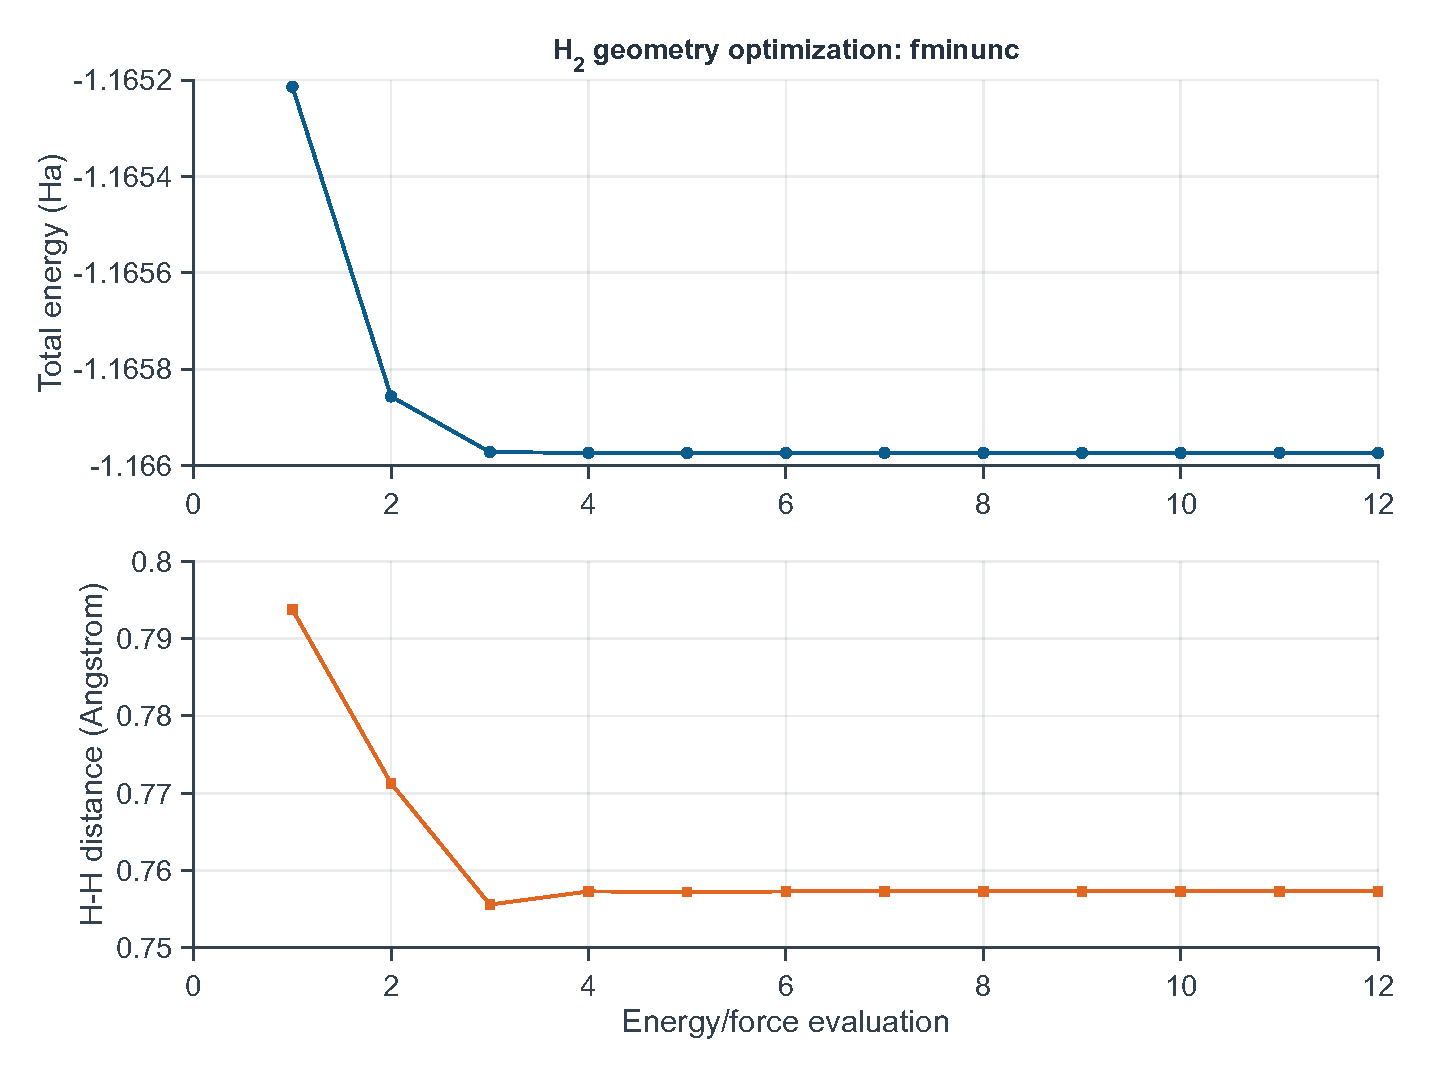
\includegraphics[width=\linewidth]{publication-assets/vector-a7002e532f8546105cf1.pdf}
\caption{氫分子幾何最佳化過程中的能量與鍵長。橫軸為能量與力的函式求值次數，包含最佳化器的試探構型。}
\label{fig:h2-relax-results}
\end{figure}

函式求值次數、電子迭代次數和幾何最佳化步數不必相同。一些方法需要試探多個位置來尋找合適步長，因此不能把日誌中出現的每一個能量值都數成一次被接受的原子移動。

\subsection{本例計算結果}

在所列條件下，fminunc 最佳化得到的最終鍵長約為 $1.43107436$ Bohr，即 $0.75729194$ Å。最終總能量約為 $-1.1659737582$ Ha，力範數約為 $5.55\times10^{-5}$ 原子單位，幾何最佳化與最後一次 SCF 均報告收斂。

與初始結構相比，鍵長略微縮短，能量降低。所得鍵長對應本例的盒尺寸、泛函、贗勢和截斷能；改變這些條件後，數值也可能變化。

最佳化記錄儲存在工作流結果中，\ui{Structure}中的原始模型保留不變。要在三維檢視器中測量最終鍵長，可匯入隨書的最佳化結構\file{examples/h2_optimized.cif}。配套指令碼也會儲存最佳化結構，供進一步分析。

\section{對稱性分析作為獨立工作流}

如果目前只想檢查結構的對稱性或推薦路徑，可以開啟二原子原胞示例專案中的 \ui{Symmetry} 模板，而不必先完成一整套電子計算。它適合在匯入晶體、建立超胞或施加形變之後，先了解結構是否符合預期。

對稱性容差描述允許多大的數值偏差仍把兩個位置或晶格引數視為相同。容差過嚴可能把檔案的小量舍入差異識別為降對稱，過寬則可能掩蓋真實畸變。對於教程提供的理想矽結構，先採用預設設定；對於實驗結構或最佳化後結構，應結合座標精度解釋分析結果。

對稱性分析描述幾何的空間關係，結構的能量與穩定性則需透過電子結構計算和原子力判斷。分析平衡結構時，將對稱性結果與最佳化記錄結合閱讀。

\section{檢視布里淵區}\label{sec:bz-workflow}
\index{Buliyuanqu@布里淵區}

布里淵區圖幫助把一維能帶路徑放回倒空間。能帶圖中的橫軸只表示沿路徑行進的距離，無法直接顯示路徑在多面體中的走向；三維布里淵區圖則同時呈現區界、高對稱點和路徑。這個練習不需要先做SCF。

% Native Online capture, 990 x 660 px after clipping, 254 ppi at 99 mm.
\begin{figure}[H]
\centering
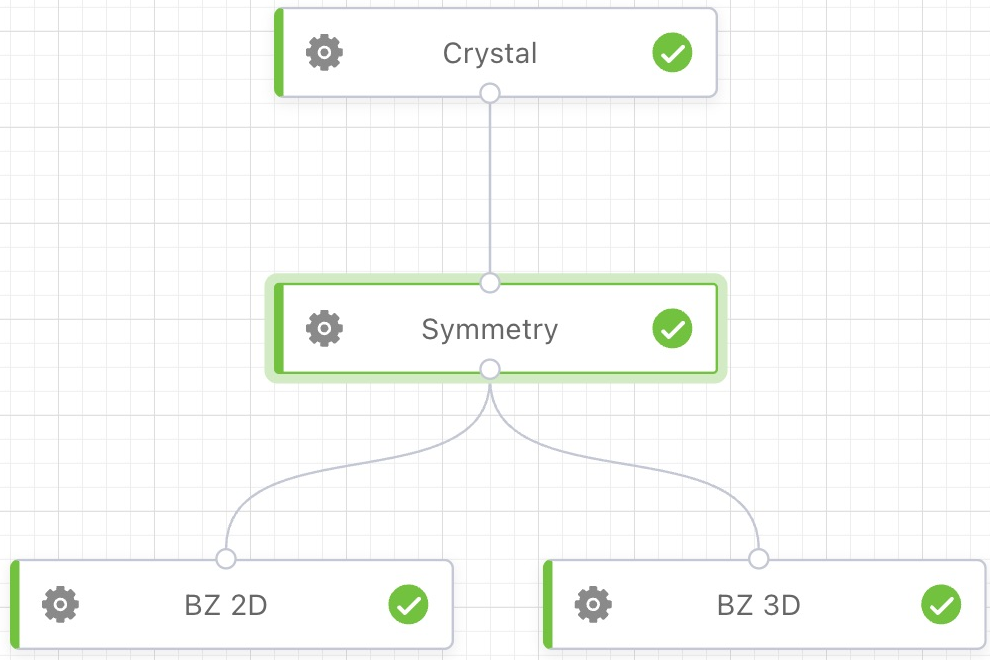
\includegraphics[width=99mm]{publication-assets/crop-7a61cf8df5b1fcc967e4.png}
\caption{\ui{Symmetry}模板的四个节点。\ui{Crystal}将晶体交给\ui{Symmetry}，分析结果分别送往\ui{BZ 2D}与\ui{BZ 3D}。运行完成后，四个节点均显示绿色完成标志。}
\label{fig:si-symmetry-online}
\end{figure}


\begin{steps}
\item 匯入\file{silicon_primitive.cif}，在專案的\ui{Structure}中確認出現二位點矽原胞。開啟\ui{主頁}的\ui{工作流}下拉選單，選擇\ui{從模板建立工作流}\,$\rightarrow$\,\ui{Symmetry}。
\item 模板包含\ui{Crystal}、\ui{Symmetry}、\ui{BZ 2D}和\ui{BZ 3D}四個節點：\ui{Crystal}提供結構，\ui{Symmetry}分析對稱性，再分別連線二維與三維圖形分支。保留這四個節點，先檢查輸入。
\item 點選\ui{Crystal}節點的齒輪開啟配置，確認任務為\ui{Build Molecule}、型別為\ui{Crystal}，在\ui{Choose imported structures}列表中只選\file{silicon_primitive}。本例保持PBE、\ui{default}贗勢、20 Ha、0 K和Nspin=1。這些欄位用於建立晶體物件，本流程沒有SCF任務。
\item 開啟\ui{Symmetry}節點配置，確認任務為\ui{Symmetry \& K-Path}，保持\ui{SymmetryThreshold}為\texttt{1e-7}、\ui{SymmetryPrecision}為\texttt{1e-5}，其餘使用預設值。再開啟\ui{BZ 3D}節點，確認\ui{Visualization Module}中的任務為\ui{Brillouin Zone 3D}；此節點沒有額外專用引數。
\item 保持這份工作流為當前活動文件，點選\ui{主頁}\,$\rightarrow$\,\ui{執行}，執行整個流程。兩個圖形分支都會生成結果，不必先執行SCF，也不必刪除\ui{BZ 2D}。
\item 在專案\ui{Results}\,$\rightarrow$\,\ui{Plots}中明確開啟\ui{BrillouinZone3D}。如果先顯示二維圖，從這裡切換至三維圖。
\item 旋轉三維檢視，辨認多面體區界、倒格軸以及$\Gamma$、X、U、W、K、L等高對稱點，觀察路徑線在前後表面之間的走向。將點標籤及路徑段與能帶教程中的同一原胞路徑對照。
\item 儲存專案；線上版使用者再將\file{.ks}專案下載到本機。需要插入報告時，使用結果圖工具條的儲存入口選擇\ui{匯出圖片}，另存影象，並儲存專案。
\end{steps}

% Original Online result export: preserve vector paths and embedded fonts.
\begin{figure}[H]
\centering
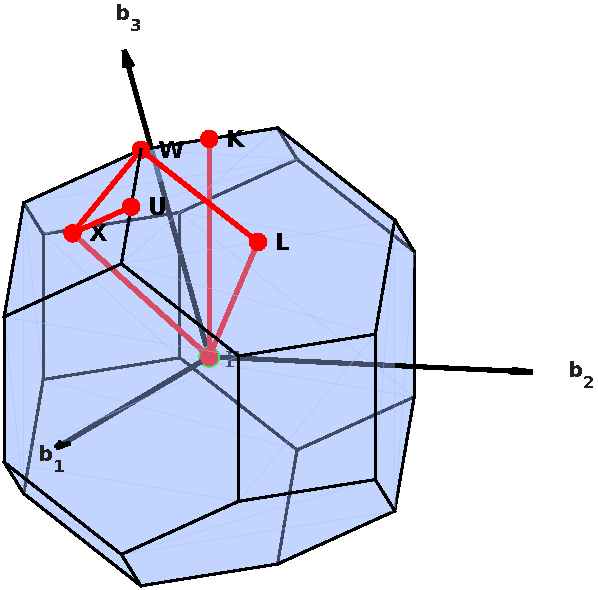
\includegraphics[width=95mm]{publication-assets/vector-cc7185e6fa1fba4c8c34.pdf}
\caption{二位点硅原胞的三维布里渊区。\ui{Symmetry}模板生成的蓝色多面体显示区界，红线连接高对称路径，黑色箭头标明倒格轴。旋转视图可以辨认$\Gamma$、X、U、W、K、L及各段的空间关系；生成布里渊区图无需SCF计算。}
\label{fig:si-bz-online}
\end{figure}


圖~\ref{fig:si-bz-online}顯示本例的三維布里淵區。隨書的\file{Si-primitive-BZ-Online-050.pdf}為向量圖，保留路徑線、點標籤與倒格軸，適合放大閱讀和插入報告。

\ui{BZ 2D}分支的任務為\ui{Brillouin Zone 2D}，按前兩個倒格矢的平面資訊作圖。對於面內倒格矢明確的二維模型，可以另建流程使用這一任務；它不是把任意三維晶體的斜截面自動變成二維材料。因此本節矽原胞以三維圖為主要觀察物件，練習二維材料時再選用標準放置的二維晶格。兩類繪圖節點的原胞、路徑和對稱性選項均在上游配置。

儲存後重新開啟專案，核對圖形、結構與高對稱路徑，再將需要的檢視用於報告。


\section{繪製能帶曲面}\label{sec:band-surface}
\index{Nengdai qumian@能帶曲面}

路徑能帶沿若干線段取樣；能帶曲面則在一張倒空間平面上取點，用曲面高度表示電子能量。它適合觀察帶邊附近的方向變化。這裡的“三維”指兩個取樣座標加一個能量座標，不是給整個布里淵區填滿三維k點，也不同於第\ref{ch:volume}章的實空間體資料。

先用\file{silicon_primitive.cif}準備一份獨立專案，保持晶體型別、PBE、default、20 Ha和原胞SCF網格；把額外能帶數設為4，使佔據帶之外還有空帶。小範圍練習採用非自旋極化的絕緣體輸入，便於辨認最高佔據帶和最低空帶。

\begin{steps}
\item 從SCF流程另存專案，保留\ui{Build Molecule → SCF}兩個節點。
\item 在後面依次連線\ui{NSCF}、\ui{Band Calculation 3D}、\ui{Band Structure 3D}。中間節點屬於Postprocessing，最後一個屬於Visualization。
\item 在NSCF節點保持本書的非自洽選項。開啟Band Calculation 3D的選項，按下表填寫中心、平面和網格。
\item 儲存流程並執行。該流程需要先完成基態求解，再在平面上進行非自洽取樣，耗時可能高於只有SCF的流程。
\item 如計算完成，檢查Results中出現的\ui{EnergyBandStructure3D}圖形。旋轉圖形觀察兩張帶邊曲面，檢查它們與取樣平面的關係，再儲存專案。
\end{steps}

\begin{table}[htbp]
\centering
\caption{能帶曲面的小網格配置示例。}
\begin{tabularx}{\linewidth}{lX}
\toprule
選項 & 輸入與含義 \\
\midrule
Center KPoint & \literalinput{[0 0 0]}，以Gamma點附近為中心。 \\
Slice Plane & XY；其他選項為XZ、YZ。 \\
Slice Plane Grid & \literalinput{[5 5]}，兩個方向各5點，共25個取樣點。 \\
Plane Grid Spacing & 0.015，控制當前任務的取樣範圍；這是倒空間引數，不是原子間距。 \\
\bottomrule
\end{tabularx}
\end{table}

本例每個方向的5個點覆蓋中心兩側各0.0375的範圍，包含兩端點；Plane Grid Spacing在這裡控制取樣範圍。需要嚴格比較兩張曲面時，同時記錄中心、平面、點數和範圍。

顯示任務選取最高佔據帶與最低空帶繪圖，能量以本次費米能為零點。兩張曲面用於觀察帶邊的色散。圖形可能不顯示座標刻度，定量分析時應讀取取樣資料，並檢查網格與範圍的收斂。


\section{準備激發態計算}\label{sec:tddft-workflow}
\index{TDDFT@TDDFT}

自洽計算得到基態電子結構。研究電子從基態受到微小擾動後可能出現的激發，需要另一類計算；TDDFT任務提供Casida方法的輸入。所需起點是已經收斂的基態電子態，並且必須包含足夠的空軌道。只把SCF流程末尾換成TDDFT，卻仍只求佔據軌道，不能建立所需的激發空間。

\subsection{為氫分子保留空軌道}

以第\ref{ch:first}章同一\file{h2.cif}為起點，另存為獨立專案，使用Molecule、PBE、default、20 Ha、Nspin=1。展開Build Molecule高階選項，把\ui{Extra bands}改為4，再執行SCF。這個中性氫分子有一個佔據的空間軌道，4條額外帶為後續選擇空軌道提供輸入；它不改變原子數量或總電荷。

在SCF之後新增Computation模組的\ui{TDDFT}節點。選擇節點並執行\ui{配置節點}，先檢視選項，再展開高階選項。

\begin{table}[htbp]
\centering
\caption{氫分子TDDFT的準備引數。}
\begin{tabularx}{\linewidth}{lX}
\toprule
欄位 & 選擇與含義 \\
\midrule
TDDFTMethod & casida，當前任務提供的方法。 \\
DiagMethod & direct，直接對角化。 \\
nvbands & 1，選用的佔據軌道數。 \\
ncbands & 4，選用的空軌道數；不得超過基態已經求出的額外軌道。 \\
nroots & 3，需要的激發態數，不能超過$nvbands\times ncbands$。 \\
Use TDA & 勾選，使用Tamm--Dancoff近似。 \\
Use IPA / Use RPA & 本例均不勾選；用於另行比較不同響應近似。 \\
\bottomrule
\end{tabularx}
\end{table}

\ui{nvbands}與\ui{ncbands}需要明確填寫，本例分別為1和4。TDDFT求解要求Nspin=1。若改變佔據軌道數、空軌道數或激發態數，應連同基態額外能帶數一起檢查。為保留簡併的一組躍遷，程式可能增加最終求解的根數；分析時以日誌和輸出陣列中的實際數量為準。

\begin{notebox}{TDDFT求解方式}
圖形介面的TDDFT節點存在引數傳遞問題，不能完成本節的激發態求解。可先按上述設定準備基態與激發空間，再在完整MATLAB\regmark{}中按下一節傳入名稱/值引數，求得激發能與躍遷向量。相關錯誤提示為\texttt{Wrong input for tddft\_input}。
\end{notebox}

\subsection{在完整 \headinglatin{MATLAB}\regmark{} 中給出顯式引數}

下面程式碼面向已經初始化KSSOLV數值環境的完整MATLAB\regmark{}，會重新進行含4條額外帶的基態計算，再明確傳入Casida引數。執行後，可檢視基態收斂狀態、激發能與躍遷向量。

\noindent\begin{minipage}{\linewidth}
\begin{lstlisting}[language=Matlab]
pseudopotential.PpType('default');
molecule = example.structure.H2();
molecule.ecut = 20;
molecule.funct = 'PBE';
molecule.extranbnd = 4;
scfOptions = options.SCF();
scfOptions.enableGPU = false;
scfOptions.enableParallelPool = false;
[molecule, H, X, scfInfo] = scf(molecule, scfOptions);
if ~scfInfo.converge
    error('Ground-state SCF did not converge.');
end
td = tddft_setup(molecule, scfOptions, H, X, ...
    'method', 'casida', 'diag', 'direct', ...
    'nvbands', 1, 'ncbands', 4, 'nroots', 3, ...
    'istda', true, 'isipa', false, 'isrpa', false);
[excitationHa, transitionVectors] = ...
    tddft_casida_direct(td, molecule);
save('h2-tddft.mat', 'excitationHa', ...
    'transitionVectors', 'scfInfo', 'td');
\end{lstlisting}
\end{minipage}

返回的激發能單位為Ha，換成eV時使用本書的單位換算。躍遷向量描述激發的軌道組合；它不直接等於一條帶有展寬和強度的吸收曲線。分析激發時，應結合基態條件、選帶數、所用近似與原始結果。


\section{讓工作流便於重複和比較}

\subsection{每條流程只承擔清楚的任務}

學習時，可以分別保留“矽 SCF”“矽能帶”“矽 DOS”三張工作流。這樣每張流程的目的都很明確，也更容易檢查執行目標。等操作熟練後，再根據需要組合流程或整理為自己的模板。

透過儲存並重新匯入 \file{.wf} 建立相同工作流後，檢查其中的結構選擇。原有設定也可能保留原始結構的關聯。如果準備計算一個新結構，先改 Build Molecule，再檢查相關模型引數。僅修改工作流名稱並不會改變計算物件。

\subsection{一個變化配一份說明}

比較引數時，名稱可以採用“矽 DOS，4×4×4”和“矽 DOS，8×8×8”這樣的簡短格式。結果說明中再記錄 SCF 網格、額外帶數、能量區間和步長。這樣既能迅速區分圖形，也保留了重現實驗所需的資訊。

專案裡舊圖不會因為節點設定改變就自動變成新條件的結果。修改設定後，需要重新執行，並確認新生成的資料與圖形屬於這次計算。整理專案時可以保留主要比較結果，刪除重複或已放棄的試算，讓專案仍然容易閱讀。

\subsection{完成一條工作流的檢查點}

儲存後重新開啟專案，依次核對結構、節點引數和計算結果，確認執行物件與方法符合說明，結果仍可閱讀。對於能帶和DOS，還應保留路徑或網格以及能量參照。
